\chapter{Credit Risk}
\label{ch:CR}

\section{Credit Risk management}
Part of the daily business of a financial institution is the credit risk assessment of existing and new customers. The result is used to decide if they want to decline or grant a credit application and, among other things, to set the required regulatory capital. Credit risk assessment is performed during the whole lifetime of an exposure. It starts with the approval of a transaction and is continuously monitored afterward. Corporate clients usually need to submit financial reports regularly, which are then analyzed by their bank advisor and credit analyst, while it is done automatically for retail customers via behavior scoring. 

The information used during the application scoring is limited because the applicant mainly provides it at the start of a new contract. It generally covers variables about their financial health, e.g., income and outstanding debt. For the behavior scoring model, internal historical data is used, for example, the borrower's payment history and credit utilization. The behavior model generally shows a better predictive performance than the application model. If a decline in financial health or behavior rating is detected, the bank may try to decrease the overdraft limit to regulate the credit risk. In the case of delayed payments, the early collection process starts, where affected customers are contacted and an alternative payment plan will be negotiated. If all interventions fail, defaulted exposures may be sold or outsourced to collection companies for further processing, like the sale of collateral. \cite[p.~7]{Witzany:2017}

\section{Default Rate and Probability of Default}
\label{sec:dr_pd}
A critical risk measure is the \acl{PD}, which is an estimate of the likelihood of a borrower failing to pay back their financial obligations in a given time period. Depending on the analyzed portfolio, the expected number of defaults can vary. In the corporate segment, individual defaults might already be seen as an indicator of a bank's failing credit assessment process and decision. In contrast, a higher number of defaults can be expected in the retail sector. On the contrary, profit is generated if the income gained from non-defaulted customers covers the loss from the defaulted portion of the portfolio. \cite[p.~2]{Witzany:2017}

\medskip
In the Capital Requirements Regulation (\ac{CRR} Article 178(1)), the definition of default is stated as:

\begin{quote}

A default shall be considered to have occurred with regard to a particular obligor when either or both of the following have taken place:
\begin{itemize}
\item[(a)] the institution considers that the obligor is unlikely to pay its credit obligations to the institution, the parent undertaking or any of its subsidiaries in full, without recourse by the institution to actions such as realising security;
\item[(b)] the obligor is more than 90 days past due on any material credit obligation to the institution, the parent undertaking or any of its subsidiaries. Competent authorities may replace the 90 days with 180 days for exposures secured by residential property or SME commercial immovable property in the retail exposure class, as well as exposures to public sector entities. The 180 days shall not apply for the purposes of point (m) Article 36(1) or Article 127.

\end{itemize}

In the case of retail exposures, institutions may apply the definition of default laid down in points (a) and (b) of the first subparagraph at the level of an individual credit facility rather than in relation to the total obligations of a borrower.

\end{quote}

A time period has to be defined in which a default event is observed, commonly a one-year observation window is used. If the customer does not default during this period, the \emph{Default\_12M} flag remains at 0. If a default occurs within the first 12 months after the start of the contract or reference point, the flag is set to 1. Notably, even if a default happens after 12 months, the flag remains at 0. An illustration is visible in Figure \ref{fig:cr_timeperiod}. The default rate per category (e.g., month, rating grade) is then calculated as the number of defaults divided by the total number of customers (Eq. \ref{eq:cr_dr}).

\begin{equation}
DR_{i} = \frac{d_{i}}{n_{i}} \label{eq:cr_dr}
\end{equation}
where:
\begin{conditions}
 d_{i}  & number of defaults in class i \\
 n_{i}  & number of observations in class i
\end{conditions}

\begin{figure}[H]
	\centering
	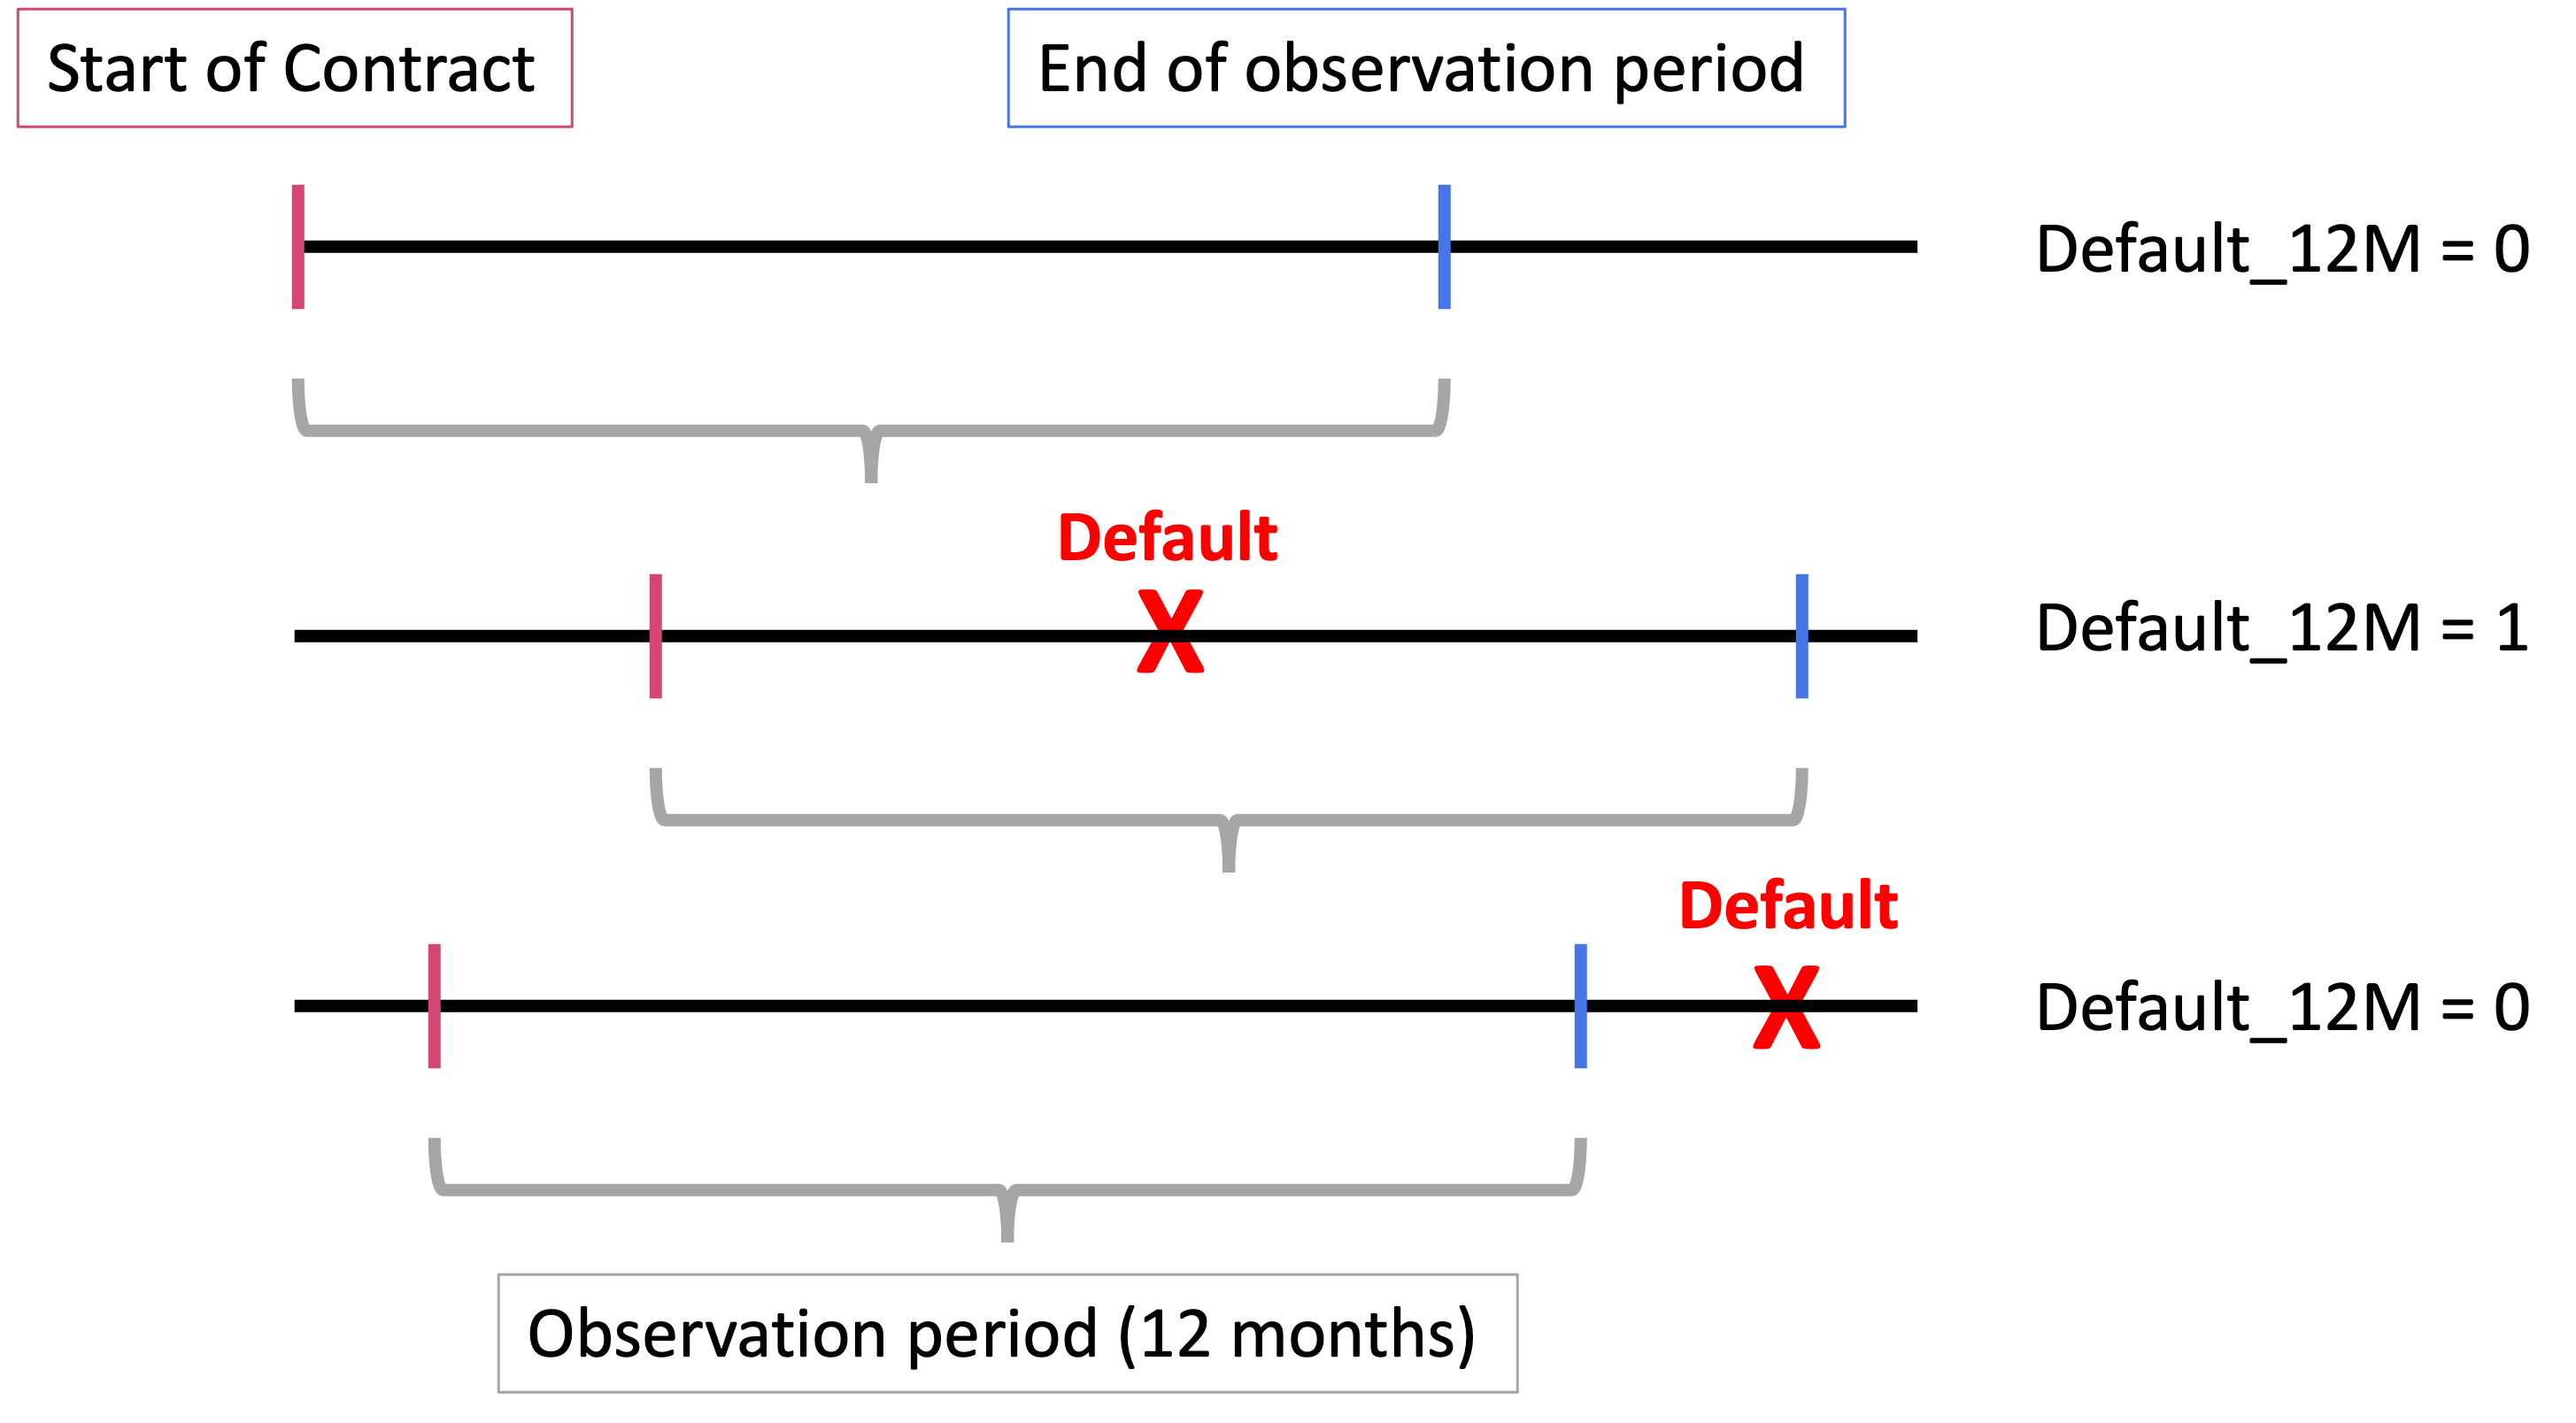
\includegraphics[width=.625\textwidth]{./CR__ObservationPeriod.png}
    \caption{Observation period, Setting of Default flag}
    \label{fig:cr_timeperiod}
\end{figure}

\section{Regulatory Framework}

\subsection{History of Regulatory Framework}

The Basel Committee on Banking Supervision, comprising 45 institutions from 28 jurisdictions since its establishment in 1945 with its headquarters in Basel, Switzerland, is dedicated to defining a high standard for risk management and internal controls and establishing a risk-sensitive calculation process of the regulatory capital for banks worldwide. The Basel Capital Accord, also known as Basel I, was first published in 1988 and set the minimum capital adequacy ratio at 8\%. Basel II, the New Capital Accord, was introduced in 2004 and implemented the three pillars encompassing the minimum capital requirements, supervisory review and market discipline. At the end of 2010, a new reform called Basel III was approved to address the variability in reported risk-weighted capital ratios during the global financial crisis, incorporating stricter regulations for the capital calculation approaches and setting a revised leverage ratio and output floor. \cite{BCBS:2023}

\subsection{Credit Risk Regulatory Capital}

The credit risk capital requirement calculation was significantly improved compared to the First Capital Accord. The total loss of a bank is split into expected and unexpected loss. The former should be covered by revenue; for the latter, a bank must allocate an appropriate level of capital. In the original approach, each exposure was assigned to one of four risk categories and then a multiplier ranging from 0-100\% was applied. Regulations now allow the \ac{SA}, Foundation or Advanced Internal Rating Based (IRB-F, IRB-A) Approach. 

The \acl{SA} defines five risk buckets for calculating regulatory capital and it also allows the use of external ratings. For the \ac{IRB} approach, internal models estimate input parameters of the regulatory formulas, which then result in risk weights for each exposure used in the calculation of the regulatory capital. The IRB-F approach only permits the estimation of the PD. In contrast, for the IRB-A approach, the risk parameters Loss Given Default, Exposure at Default, Conversion Factor and Effective Maturity are additionally derived from internal models. While the corporate segment allows for both IRB-F and IRB-A approaches, the retail portfolio is limited to the IRB-A approach. \cite[15-17]{Witzany:2017} 

\subsection{Machine Learning for IRB models}
The integration of advanced machine learning models in the banking industry is in its early stages, as financial institutions struggle with uncertainties regarding the application of requirements outlined in the \acl{CRR} and other legal frameworks such as the \ac{GDPR} and the Artificial Intelligence (AI) Act. Notably, the AI Act designates credit scoring as a high-risk use case, given its potential impact on an individual's access to financial resources. Within the banking sector, machine learning models find additional application in areas like fraud detection, transaction clustering and real-time monitoring of payments. Decision trees are commonly utilized in the development of \ac{IRB} models for variable selection, clustering processes and as model challengers in subsequent validation. 

Financial institutions encounter challenges related to overfitting and interpretation of machine learning models, compounded by a shortage of credit risk analysts equipped with the necessary skills to navigate these complexities. Overfitting issues are particularly pronounced in low default portfolios, where the training of advanced models necessitates extensive data for robust outcomes. Credit analysts with expertise in overcoming these challenges, including hyperparameter tuning, interpretation methods and evaluating output stability and bias, are scarce. Another significant barrier lies in the acceptance of more complex models, requiring a solid understanding from all participants, especially senior management, stakeholders and the sales force. Additionally, one of the objectives of employing machine learning models is leveraging unstructured data; however, \ac{GDPR} Article 9 prohibits the use of personal data, necessitating additional efforts to analyze the compliance of input information. Despite these challenges, the ongoing integration of advanced machine learning models in the banking sector signals a transformative shift, with the need for collaborative efforts to navigate regulatory requirements, enhance analytical capabilities and foster a deeper understanding among key stakeholders.\cite[pp.~4-7, 9, 11, 13]{EBA:2023}